\chapter{The CMS experiment at LHC}
\label{cap2}
\textit{The data used in this analysis has been collected by the Compact Muon detector. It is one of the main experiments located at the Large Hadron Collider at CERN. This chapter provides a general description of the accelerator system and of  the detector   involved in producing and
recording the data. In particular I have been involved in the CMS data taking and in data validation operation since 2016, Fig.~\ref{int_lumi_cumulative_pp_1}.}

\section{The Large Hadron Collider}
The Large Hadron Collider (LHC)~\cite{Pettersson:291782}  at CERN,
which started operations in 2008, is the largest and most powerful hadron collider ever built. Installed in the
underground tunnel which housed the Large Electron Positron Collider (LEP),
in operation until 2000, the LHC accelerator
has approximately the shape of a circle with a length of about 27 km
and is located underground at a depth varying
between 50 m to 175 m, straddling the Franco-Swiss border near Geneva. It is designed
to collide two 7 TeV counter-circulating beams of protons resulting in a center-of-mass
energy of 14 TeV, or two beams of heavy ions, in particular lead nuclei at an energy of
2.76 TeV/nucleon in the center-of-mass frame.
The transition from a leptonic collider to a hadronic collider entailed the following
advantages: first, it has been possible to build a machine that having the same size of the
previous one (and therefore accommodated in the same tunnel,
substantially reducing the cost and time of construction), could reach
a higher energy in the center-of-mass
frame. This is due to the much lower amount of energy loss through synchrotron radiation
emitted by the accelerated particles, that is proportional to the fourth power of the ratio
E/m between their energy and their mass. Secondly, the composite structure of protons
compared to the elementary structure of electrons allows LHC to be able to access simultaneously a wider energy spectrum, despite the production of many low energies particles in a complex environment. This feature is particularly important for a machine dedicated
to the discovery of “new” physics.

A schematic description of the accelerator complex installed at CERN is shown in Fig.~\ref{lhc}
The acceleration is performed in several stages. The protons source is
a Duoplasmatron: the protons are obtained by removing electrons from a
source of hydrogen gas 
and then sent to the LINAC2, a 36 m long linear accelerator which generates a pulsed
beam with an energy of 50 MeV using Radio Frequency Quadrupoles (RFQ) and focusing
quadrupole magnets. The beam is subsequently sent to the Proton Synchrotron Booster
(PSB), a circular accelerator consisting of four superimposed synchrotron rings with a
circumference of about 160 m, which increases the proton energy up to 1.4 GeV. Then,
protons are injected into the Proton Synchrotron (PS), a single synchrotron ring with a
circumference of about 600 m where the energy is increased to 25 GeV. The sequential combination of these two synchrotrons also allows to create a series of protons bunches
interspersed by 25 ns (i.e. at the frequency of 40 MHz) as required for the final correct
operation of LHC. The final proton injection stage is the Super Proton Synchrotron (SPS),
a synchrotron with a circumference of approximately 7 km where protons reach an energy
value of 450 GeV. Subsequently, protons are extracted and injected into the LHC ring
via two transmission lines, to generate two beams running in opposite directions in two
parallel pipes and which are accelerated up to the energy of interest.

The beams collide
at four interaction points where the four main experiments are
located: ALICE, ATLAS, CMS and LHCb. Two small experiments, TOTEM and
LHCf, which focus on forward particles, have also been installed near,
respectively, CMS and ATLAS.
The 7 TeV per-beam-energy limit on the LHC
is not determined by the electric field generated by the radiofrequency cavity but by the
magnetic field necessary to maintain the protons in orbit, about 8.3 T, given the current technology
for the superconducting magnets.
\begin{figure}
\centering
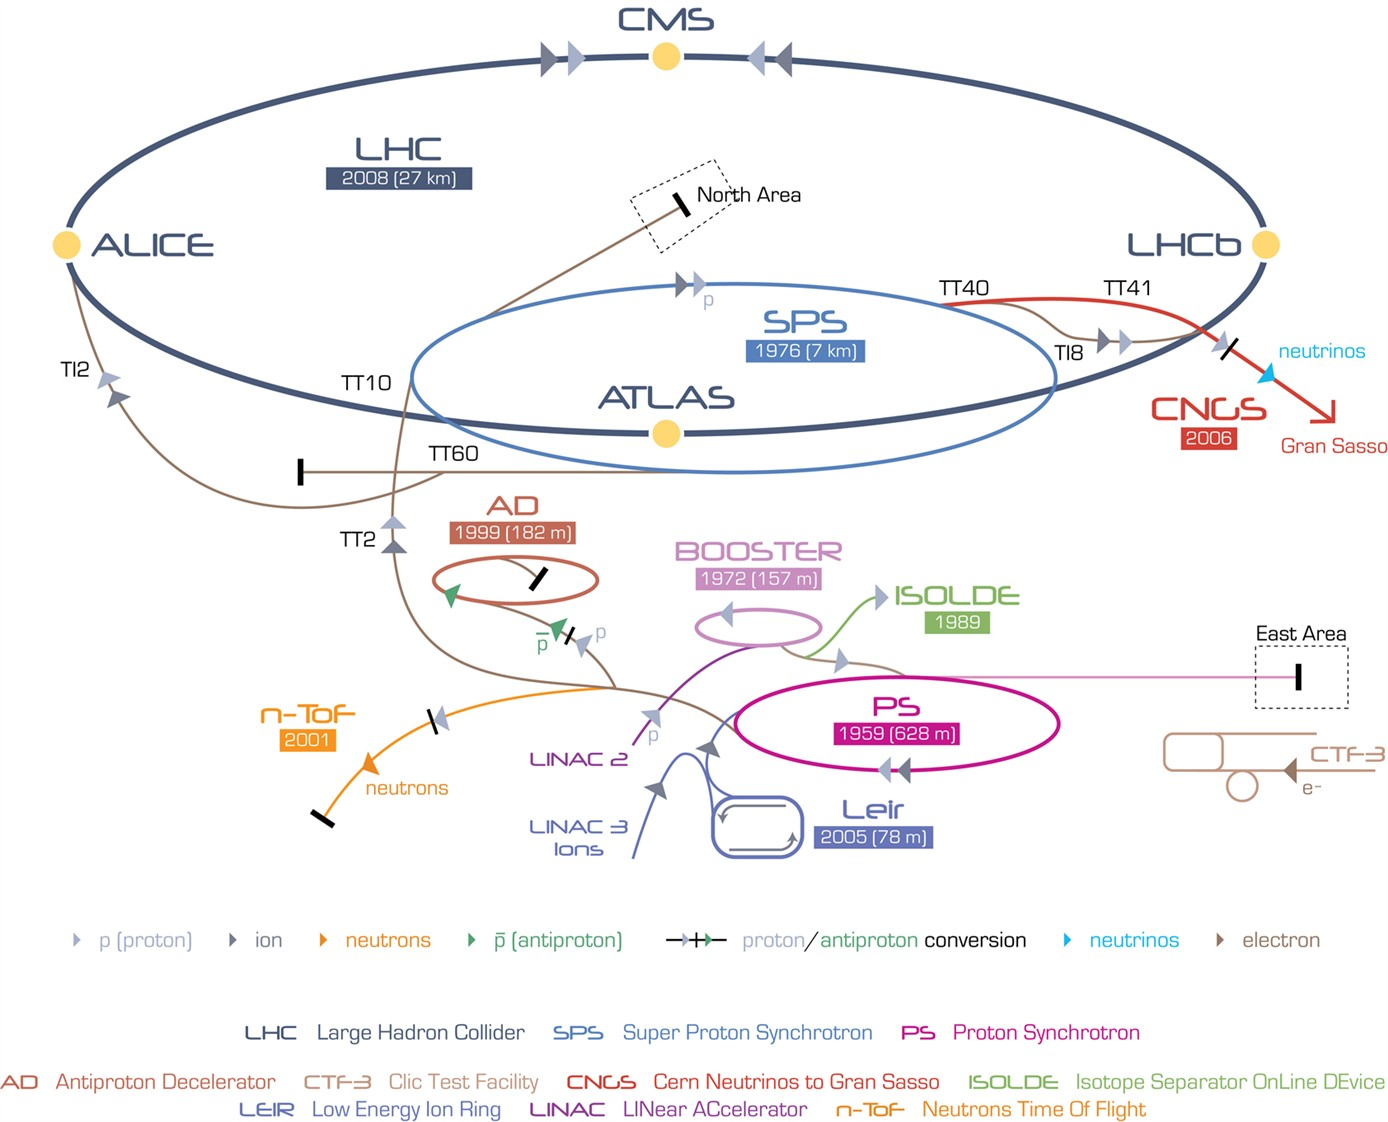
\includegraphics[scale= 0.6]{../Cap2/lhc_cern}
\caption{Schematic layout of the accelerator complex installed at CERN.}
\label{lhc}
\end{figure}

One of the most important parameter of an accelerator is the
{\em instantaneous luminosity} $\mathcal{L}$. For a given process having a cross section $\sigma$, the
instantaneous luminosity $\mathcal{L}$ is defined by the relation
\begin{equation}
N= \mathcal{L} \sigma, \end{equation}
where $N$ is the rate of occurrence of the process. Then the {\em
  integrated luminosity} $L$ is defined as the integral of the
instantaneous luminosity over time, i.e.
\begin{equation}
L=\int \mathcal{L}  dt.
\end{equation}

\section{The Compact Muon Solenoid experiment}
The Compact Muon Solenoid (CMS)  is a general purpose detector
optimized for the analysis of the 
proton-proton interactions with the expected energy and luminosity of
the LHC. CMS is able to accurately identify muons, electrons, photons
and hadrons. It
has been designed to investigate a wide range of physics, with the search for the Higgs
boson as one of the main highlights. Search for new physics is also an important goal of the
experiment, as well as top physics and, of course, Standard Model precision measurements.
%Although it has the same scientific goals as the ATLAS experiment, it uses different
%technical solutions and a different magnet-system design.
The collaboration that run the CMS experiment is one
of the largest international scientific community in history, involving more than 4000
people (particle physicists, engineers, technicians, students and support staff) from about
180 universities and research institutes in more than 40 countries.
The experimental apparatus is placed in a cavern 100 m underground in
the area called Point 5 (an old LEP access point) near the village of
Cessy, in France. 

The coordinate system used in CMS is a right-handed Cartesian system, having the origin
in the nominal beam collision point inside the detector. The x-axis points radially towards
the center of the LHC ring, the y-axis is directed upwards along the vertical and the z-axis 
is oriented along the direction of the beams, along the counter-clockwise direction of
the ring if seen from above. The cylindrical symmetry of CMS design and the invariant
description of proton-proton physics suggest to define also a coordinate system based on
pseudo-angular coordinates, given by the triplet ($r$, $\phi$, $\eta$) where $r$ is the distance from
the $z$-axis, $\phi$ is the azimuthal angle measured on the $x-y$ plane starting from the $x$-axis
and $\eta$ is the pseudorapidity (please refer to Appendix~\ref{psr}
for more details).

The CMS detector, shown in Fig.~\ref{cms}, is 21.6~m long, has a diameter of 15~m and a
weight of about 12,500 tons. The constructive element that characterizes the experiment
is a solenoidal superconducting magnet which produces an internal constant magnetic
field of 3.8 T along the direction of the beams. The CMS detector is designed as a
dodecagonal base prism. The central part of the prism, named barrel, contains several
layers of detectors with quasi-cylindrical symmetry, coaxial with respect to the direction of the
beams. A set of detector disks, called endcaps, close the detector at its ends, to ensure hermeticity. 
\begin{figure}
\centering
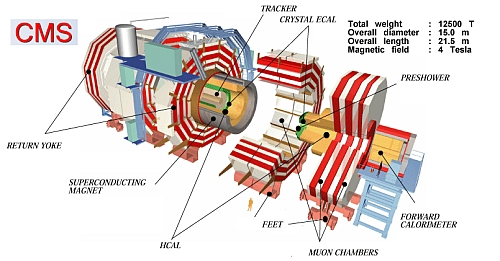
\includegraphics[scale= 0.21]{../Cap2/cms} %CMSnc
\caption{An exploded view of the CMS detector with all subdetectors.}
\label{cms}
\end{figure}

From the inner region to the outer one, the various components of CMS are:
\begin{itemize}
\item Silicon Tracker: it is placed in the region $r$ < 1.2 m and $|\eta|$ < 2.5. It consists of
a silicon pixel vertex detector and a surrounding silicon microstrip detector, with a
total active area of about 215 m$^2$. It is used to reconstruct charged particle tracks
and vertices;
\item Electromagnetic Calorimeter (ECAL): it is placed in the region 1.2~m $< r <$
1.8~m and $|\eta|$< 3. It consists of scintillating crystals of lead
tungstate  and it is used to measure the direction and energy of photons and electrons;
\item Hadron Calorimeter (HCAL): it is placed in the region 1.8 m $< r <$ 2.9~m and
$|\eta|$ < 5. It consists of brass layers alternated with plastic scintillators and it is used
to measure the direction and the energy released by the hadrons produced in the
interactions;
\item Superconducting Solenoidal Magnet: it is placed in the region 2.9~m $< r <$
3.8 m and  $|\eta|$< 1.5. It generates an internal uniform magnetic field of 3.8~T along
the direction of the beams, necessary to deflect the charged particles in order to
allow a measurement of their momentum through the curvature observed in the
tracking system. The magnetic field is closed with an iron yoke 21.6~m long with a
diameter of 14~m, where a residual magnetic field of 1.8~T is present, opposite
in direction with respect to the 3.8~T field;
\item Muon System: it is placed in the region 4 m $< r < 7.4$ m and $|\eta|$ < 2.4. It consists
of Drift Tubes (DT) in the barrel region and Cathode Strip Chambers (CSC) in the
endcaps. A complementary system of Resistive Plate Chambers (RPC) is used both
in the barrel and in the endcaps. This composite tracking system for muons is used
to reconstruct tracks released by muons that pass through it. The muons chambers
are housed inside the iron structure of the return yoke that encloses the magnetic
field.
\end{itemize}

\subsection*{The Tracker}
The silicon tracker is the detector closest to the beams collision point. Its goal is
the high resolution reconstruction of the trajectories of charged particles originating
from the collision region and the identification of the position of secondary vertices
produced by particles with a short mean life time (in particular hadrons containing the
b quark, that decay after few hundreds of $\mu$m). The events produced in the proton-
proton collisions can be very complex and track reconstruction is a
challenging pattern
recognition problem. Indeed, at the nominal instantaneous luminosity of operation,
an average of about 20 pile-up events overlapping to the event of interest are expected,
leading to about 1000 tracks to be reconstructed per event.

In order to ease the pattern recognition, two requirements are fundamental:
a low occupancy detector and a large redundancy of the measured points (hits) per track.
The first requirement is achieved building a detector with high granularity. The
redundancy of the hits is instead achieved having several detecting layers, and is
necessary to reduce the ambiguity on the assignment of the hits to a given track.
Nevertheless, the amount of tracker material has to be as low as possible, in order to
avoid jeopardizing the measurement of the particle trajectory. An excessive amount
of material would indeed deteriorate the measurement, mainly because
of multiple scattering and energy loss for charged particles,
bremsstrahlung for electrons and nuclear interactions for hadrons.
The outer detectors such as ECAL are influenced by the material as
well, for example because of the increased probability 
for a photon to convert to an electron-positron pair in the tracker
material.

For these
reasons, the tracker layers are limited in number and thickness. The tracker comprises
a large silicon strip detector with a small silicon pixel detector inside it. In the central
$\eta$ region, the pixel tracker consists of three co-axial barrel layers at radii between
4.4~cm and 10.2~cm and the strip tracker consists of ten co-axial barrel layers extending
outwards to a radius of 110~cm. Both subdetectors are completed by endcaps on either
side of the barrel, each consisting of two disks in the pixel tracker, and three small
plus nine large disks in the strip tracker. The endcaps extend the acceptance of the
tracker up to $|\eta|$<2.5. A three-dimensional schematic view of the tracker is shown in
Fig.~\ref{trk}, while in Fig.~\ref{fig_cmstracker} a pictorial representation of a slice of the tracker is displayed,
showing the various layers of the subdetectors.
The whole tracker has a cylindrical shape with a length of 5.8~m and a diameter
of 2.5~m, with the axis aligned to the beams direction. The number of hits
per track is 12-14, allowing high reconstruction efficiency and low rate of fake tracks.

\begin{figure}
\centering
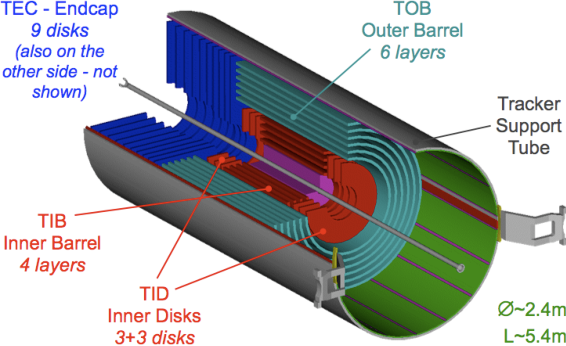
\includegraphics[scale= 0.5]{../Cap2/trk}
\caption{Three-dimensional schematic view of the CMS silicon tracker.}
\label{trk}
\end{figure}

\begin{figure}
\centering
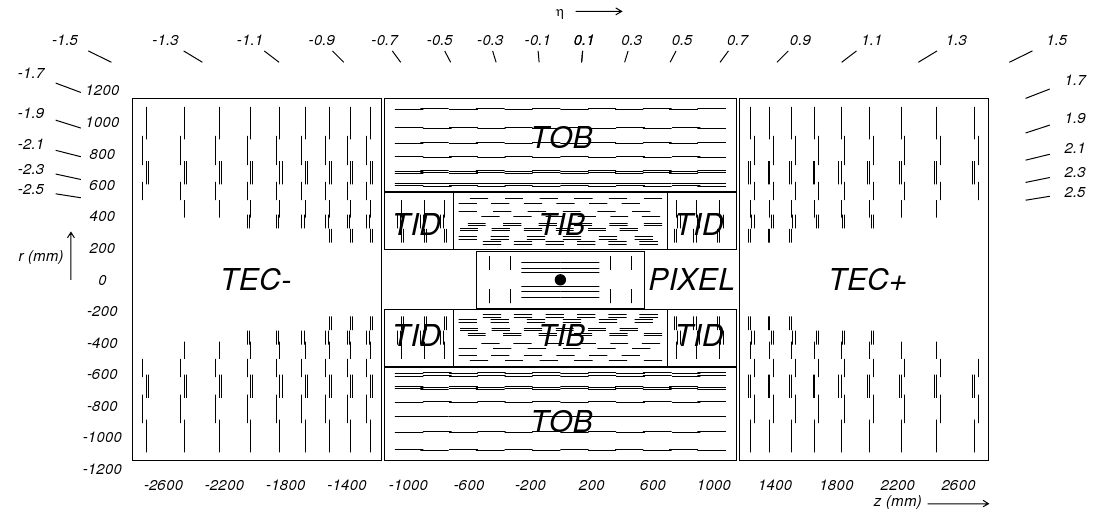
\includegraphics[scale= 0.3]{../Cap2/fig_cmstracker}
\caption{Pictorial view of a tracker slice in the r-z plane. Pixel modules are shown in
red, single-sided strip modules are depicted as black thin lines and strip stereo modules are
shown as blue thick lines.}
\label{fig_cmstracker}
\end{figure}

\paragraph*{The Pixel Vertex Detector} The pixel vertex detector is mainly used in CMS as a starting point for
the reconstruction of tracks and is essential for the reconstruction of the primary vertex
(PV) and any possible secondary vertices. It is placed in the region closest to the collision
point, where the particle flux is maximum. It covers the region $|\eta|$ < 2.5 and is composed
of a central part (barrel) and by two forward parts (endcaps).

The barrel consists of
three concentric cylindrical sectors 53~cm long, located at an average distance r of 4.4~cm,
7.3~cm and 10.2~cm. Each half-cylinder is made up of ladders and half ladders that serve
as support and cooling structure for the pixel modules, with each ladder containing 8
modules. In total, the barrel is composed of 768 modules.

Each endcap is composed of
two disks placed at a distance of 34.5~cm and 46.5~cm from the nominal beams impact
point. They cover a radius $r$ in a range between 6~cm and 15~cm in such a way that each
track within the detector acceptance passes through at least two layers. Each disk is
divided into 24 segments, on each of which 7 modules of different sizes are mounted, for
a total of 672 modules on all the endcaps.

A module is composed by a silicon sensor with a thickness of
250 $\mu$m and the corresponding readout chips. In
order to optimize the reconstruction of track and vertices near the
interaction point, the sensor is segmented into rectangular pixels
with a size of $150\times100\mu$m$^2$, with the 100$\mu$m side 
oriented along the $r \phi$ direction in the barrel region and along the $r$ direction in the endcap
region. The hit position resolution is about 10-15 $\mu$m in the barrel and
about 15 $\mu$m in the endcaps.

\paragraph*{The Silicon Microstrip Detector} In the region of the detector that is more than 20~cm far from the beam, the flux of
charged particles is sufficiently limited to allow the use of a silicon microstrip detector. Overall, this detector (Silicon
Strip Tracker, SST) consists of 15400 elementary units or modules,
composed by one or two sensors stuck onto a support of carbon fiber together with the readout
electronics. In some of the layers and in the innermost rings, special
double-sided modules are able to provide accurate three-dimensional
position measurement of the charged particle hits by having the two silicon
sensors rotated in order to have strips forming an angle of 100 mrad. 
This “stereo” combination, although of lower resolution, is preferable
compared to a pixel segmentation because it requires a lower number of
readout channels.  

The
silicon microstrip tracker is 5.4 m long, extending up to a distance of 1.1 m from the axis
of the beams. It consists of a barrel and two endcaps and it is divided into four distinct
parts, TIB and TOB, and TID and TEC.


\subsection*{The Electromagnetic Calorimeter (ECAL)}
The main function of an electromagnetic calorimeter is to identify
electrons and photons measuring accurately their direction and energy. The electromagnetic calorimeter (Fig.~\ref{ecal_all}) of
CMS (ECAL, Electromagnetic CALorimeter)  is a homogeneous calorimeter with
cylindrical geometry, whose active elements are scintillating crystals of lead tungstate (PbWO$_4$)
with a truncated pyramidal shape. It consists of an ECAL Barrel (EB) with 61200 crystals
and two ECAL Endcaps (EE) containing 7324 crystals each.
Crystals are grouped into 5 × 5 matrices called towers.

The barrel has an inner radius of
129 cm, a length of 630 cm and it extends in the region $|\eta|$ < 1.479. Crystals in the ECAL
barrel have the following dimensions: 22$\times$22 mm$^2$ at the front face, 26 $\times$ 26 mm$^2$ at the
rear face, and a length of 23~cm, corresponding to 25.8 $X_0$. Each submodule, consisting
in a 5 $\times$ 2 crystals arrays mounted on a glass fiber structure, forms the elementary unit of
EB.
%The granularity of a single crystal is about 1 degree.
To avoid that cracks might align with
particle trajectories, the crystal axes are tilted by 3 degrees with respect to the direction from
the interaction point, both in the $\eta$ and $\phi$ direction.

Each endcap covers the region 1.479 < $|\eta|$ < 3 and is formed by two semicircular halves
of aluminum called dees. Crystals in endcaps have a length of 22 cm and frontal area
equal to 28.6 × 28.6 mm$^2$. They are arranged in supercrystals with 5 $\times$ 5 elementary unity.
Unlike the crystals in the barrel, arranged in a $\eta - \phi $ geometry, the endcap crystals are
arranged according to a $xy$ geometry.

Two preshower detectors are placed in front of the endcaps in order to disentangle the
showers produced by a primary $\gamma$ from those produced by a primary $\pi_0$. This detector,
which covers the region 1.653 <  $|\eta|$ < 2.6, is a sampling calorimeter and it consists of two
disks of lead converters  that start the electromagnetic
shower of the incident photon/electron, alternating with two layers of silicon microstrip
detectors in which a measurement of the released energy and the identification of the
shower profile are performed. The strips are arranged orthogonally in the two planes,
according to a $xy$ configuration.
\begin{figure}
\centering
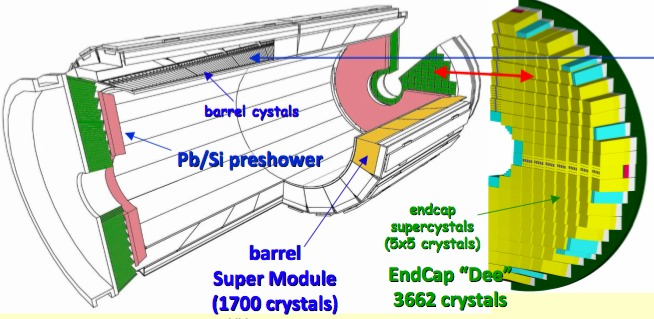
\includegraphics[scale= 0.5]{../Cap2/ecal_all}
\caption{Schematic representation of the electromagnetic calorimeter ECAL.}
\label{ecal_all}
\end{figure}

The choice of the PbWO$_4$ crystals as scintillating material for ECAL is due to several
reasons. First, the high-density, the short radiation length  and the
reduced Molière radius (R$_M = 2.2$~cm) allow to build a compact and
high granularity calorimeter. Furthermore, the 15 ns scintillation
decay time allows to collect about 80\% of the emitted light during
the 25 ns that exist between two consecutive bunch crossings in the
LHC. Finally, the PbWO$_4$ crystals have a 
good intrinsic radiation hardness and therefore they can operate for years in the hostile
LHC environment, with a modest deterioration in performance. The main disadvantage
of these crystals is the low light yield  which makes an internal
amplification for the photodetectors necessary. This is achieved through the use of silicon
avalanche photodiodes  in barrel and single stage photomultipliers  in the endcaps, both resistant to the radiation and to the strong
magnetic field of CMS.

The energy resolution of a homogeneous calorimeter is usually expressed by the sum
in quadrature of three terms, according to the formula,
\begin{equation}
\frac{\sigma_e}{E}=\frac{a}{\sqrt{E}} \bigoplus \frac{b}{E} \bigoplus c \; ,
\end{equation}
The stochastic term $a$ is dominant at low energies: it includes the contribution
of statistical fluctuations in the number of photoelectrons generated and collected.
The noise term $b$ includes contributions from the electronic noise,
both due to the photodetector and to the preamplifier, and from pileup
events. 
The constant term $c$, dominant at high energies, takes into account several contributions:
the stability of the operating conditions (in particular of temperature and voltage), the
presence of dead material in front of the crystals and the rear leakage of the electromagnetic 
shower, the longitudinal non uniformity of the crystal light yield, the intercalibration
errors and the radiation damage of the crystals.
The ECAL barrel energy resolution for electrons in beam tests has been measured 
to: $a=2.8\%$~GeV$^{-1/2}$, $b=12\%$~GeV, $c\approx$0.3\%, where the energy E is measured in GeV.

\subsection*{The Hadronic Calorimeter (HCAL)}
The hadronic calorimeter HCAL (Hadronic CALorimeter ) complements the
electromagnetic calorimeter to build up a complete calorimetric system for the jet energy and
direction measurement. Furthermore, thanks to its hermeticity, it can provide a measurement 
of the properties of non-interacting particles, such as neutrinos, by measuring the
missing energy deposited in the transverse plane, $E_T^{Miss}$ or MET.

The CMS hadronic calorimeter is
a hermetic sampling calorimeter that covers the region $|\eta|$ < 5. As shown in Fig.~\ref{hcal},
it is divided into four subdetectors: HB (Barrel Hadronic Calorimeter ), located in the
barrel region inside the magnet, extending up to pseudorapidities  $|\eta|\sim$1.4; HE (Endcap
Hadronic Calorimeter), situated in the endcaps region inside the magnet, extends in the
pseudorapidity region 1.3~$<|\eta|<$~3, partially overlapping the HB coverage; HO (Outer
Hadronic Calorimeter, also called tail-catcher, placed along the inner wall of the magnetic 
field return yoke, just outside of the magnet; HF (Forward Hadronic Calorimeter),
a sampling calorimeter made of quartz fibers sandwiched between iron absorbers,
consisting of two units placed in the very forward region (3 ~$<|\eta|<$~5) outside the magnetic coil. 
At the passage of charged particles, Cherenkov light is emitted in the quartz fibers 
and this light is detected by radiation resistant photomultipliers.

In order to maximize particle containment for a precise missing transverse energy
measurement, the amount of absorber material was maximized, reducing therefore the
amount of the active material. Since HCAL is mostly placed inside the magnetic coil,
a non-magnetic material like brass was chosen as absorber. HB and HE are therefore
made with brass absorber layers interleaved with plastic scintillators
coupled to wavelength shifting optical fibers which transmit the light to the HPD (Hybrid
Photodiodes) photodetectors.
\begin{figure}
\centering
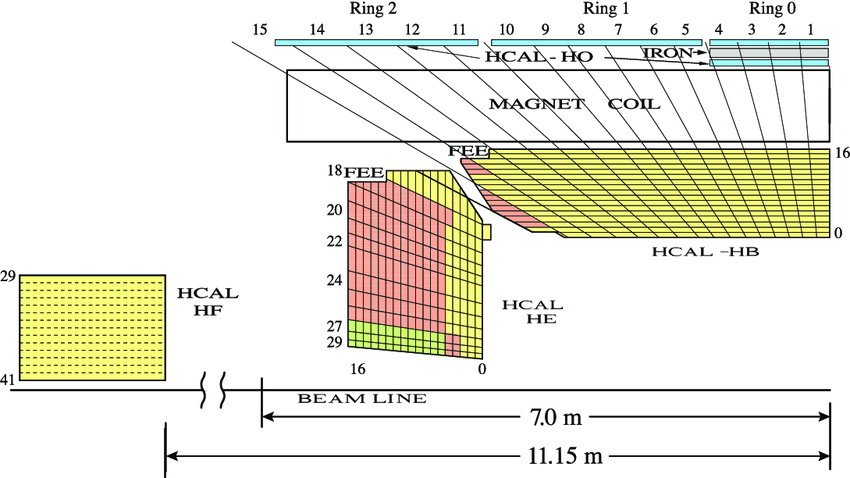
\includegraphics[scale= 0.4]{../Cap2/hcal}
\caption{A schematic $rz$ view of a quadrant of the CMS hadronic calorimeter HCAL.}
\label{hcal}
\end{figure}


\subsection*{The Solenoidal Magnet}
The CMS magnet (shown in Fig.~\ref{magnetarrival}) houses the tracker, the electromagnetic and the hadronic
calorimeters and is the biggest superconducting solenoid ever built in the world. The solenoid
achieves a magnetic field of 3.8~T in the free bore of 6~m in diameter and 12.5~m in length.
The energy stored in the magnet is about 2.6~GJ at full current. The superconductor is
made of four Niobium-Titanium layers. In case of a quench, when the magnet loses its
superconducting property, the energy is dumped to resistors within 200 ms. The magnet
return yoke of the barrel is composed by three sections along the z-axis; each one is
split into 4 layers (hosting the muon chambers in the gaps). Most of the iron volume is
saturated or nearly saturated, and the field in the yoke is about half (1.8 T) the
field in the central volume.

\begin{figure}
\centering
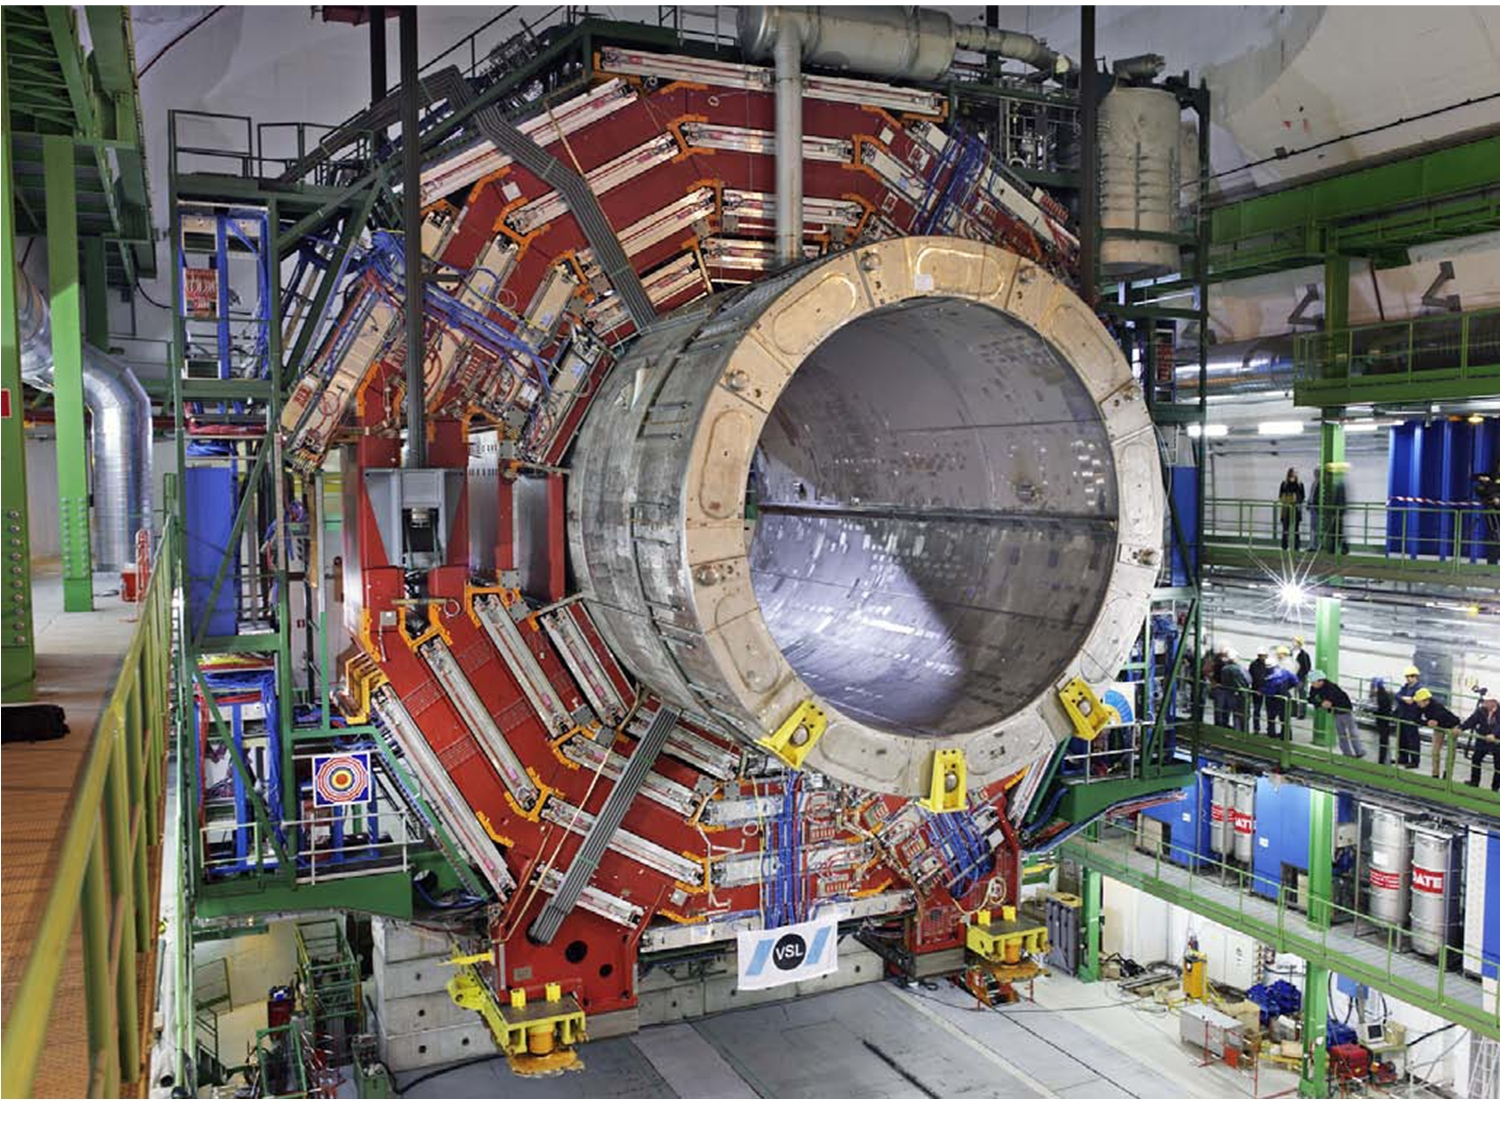
\includegraphics[scale= 0.35]{../Cap2/magnet}
\caption{Arrival of the magnet in the tunnel on February 28, 2007.}
\label{magnetarrival}
\end{figure}

\subsection*{The Muon chamber}
The CMS Muon System  is dedicated to the identification of muons and
measurement of their transverse momentum, $p_T$, in combination with the tracker. Furthermore, it provides a time measurement
of the bunch-crossing and also works as trigger for events involving muons. Momentum
measurement, in the muon system, is determined by the muon bending angle at the exit
of the 3.8 T coil, considering the interaction point as the origin of the muon. Up to $p_T$
values of 200 GeV, the resolution of the muon system is dominated by multiple scattering
and the best resolution is rather given by the silicon tracker, as
shown in Fig~\ref{muon_res}. The system is placed outside
the magnetic coil, embedded in the return yoke, to fully exploit the 1.8 T return flux. It
consists of three independent subsystems, as shown in Fig.~\ref{muon_c}: drift tubes (DT), cathode strip chambers (CSC) and resistive plate
chambers (RPC). The DT and the CSC provide an excellent spatial resolution for the
measurement of charged particle momentum; the RPC are used for trigger issues because
of the very good timing. The active parts of the muon system are hosted into stations
which are interleaved by the iron layers of the return yoke of the magnet. 

\begin{figure}
\centering
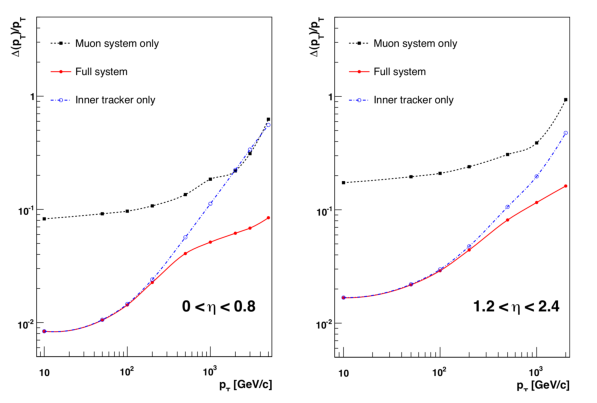
\includegraphics[scale= 1.2]{../Cap2/muon_res}
\caption{Muon transverse momentum resolutions for the tracking system. On the left the barrel zone. On the right the endcap.}
\label{muon_res}
\end{figure}
\begin{figure}
\centering
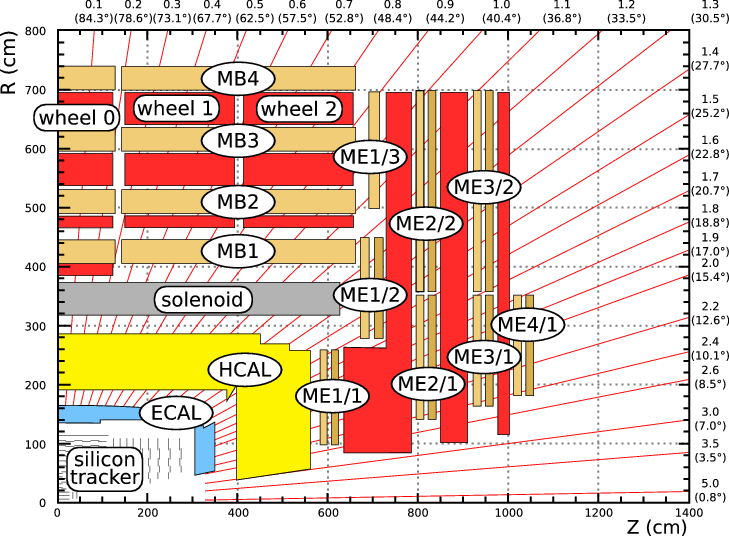
\includegraphics[scale= 0.4]{../Cap2/muon}
\caption{Schematic overview of the muon chambers.}
\label{muon_c}
\end{figure}


\subsection*{Trigger and Data Acquisition}
LHC can produce interactions at 40 MHz frequency, but only a small fraction of these
events can be written on disk. On one hand the speed at which data can be written
to mass storage is limited, on the other hand the vast majority of events produced is
not interesting, because it involves low transverse momentum interactions (minimum bias
events). Thus, a trigger system is needed to select interesting events at the highest possible
rate. The maximum rate of events written on disk is about 800 Hz. CMS has chosen a
two-level trigger system, consisting of a Level-1 Trigger (L1)  and a High Level Trigger
(HLT).
Level-1 trigger runs on dedicated processors, and accesses coarse level granularity information 
from calorimetry and muon system. A L1 Trigger decision has to be taken for
each bunch crossing within 3.2 $\mu$s. Its task is to reduce the data flow from 40 MHz to
about 100 kHz. The High Level Trigger is responsible for reducing the L1 output rate down to a maximum
rate of the order of 1 kHz. The HLT code runs on a farm of commercial processors and can access the full granularity information of all the subdetectors.

\section{Data samples and future plans}
The first proton beam circulated in the LHC on September 2008, after more than a decade of construction and installation.
An incident occurred in two magnets, causing the release of helium into the tunnel
and mechanical damage. After that, in March  2010 started the Run-I, a fruitful data taking era that lasted until
2012.  It was decided not to operate the LHC at its design parameters, and proton proton collisions
took place at a centre of mass energy of 7 TeV and 8 TeV. The amount of recorded data (in CMS) in this period is reported in Fig.~\ref{int_lumi_cumulative_pp_1}.
At the end of 2012, LHC operations halted for two years due to the first long shutdown (LS1).
In 2015, with centre-of-mass energy of 13 TeV, the proton-proton collision restarted (Run-II) and, in the 2016,  LHC was ready to deliver a large dataset to the experiments.
The data collected in 2016 are used in the high mass analysis that is
the subject of this thesis. Overall, the data correspond to 35.9
fb$^{-1}$ of data validated for the physics analyses. The 2016 LHC operations can be
grouped into several time-periods,  
labelled with a letter from A to H, corresponding to slightly different conditions of data taking.
\begin{figure}
\centering
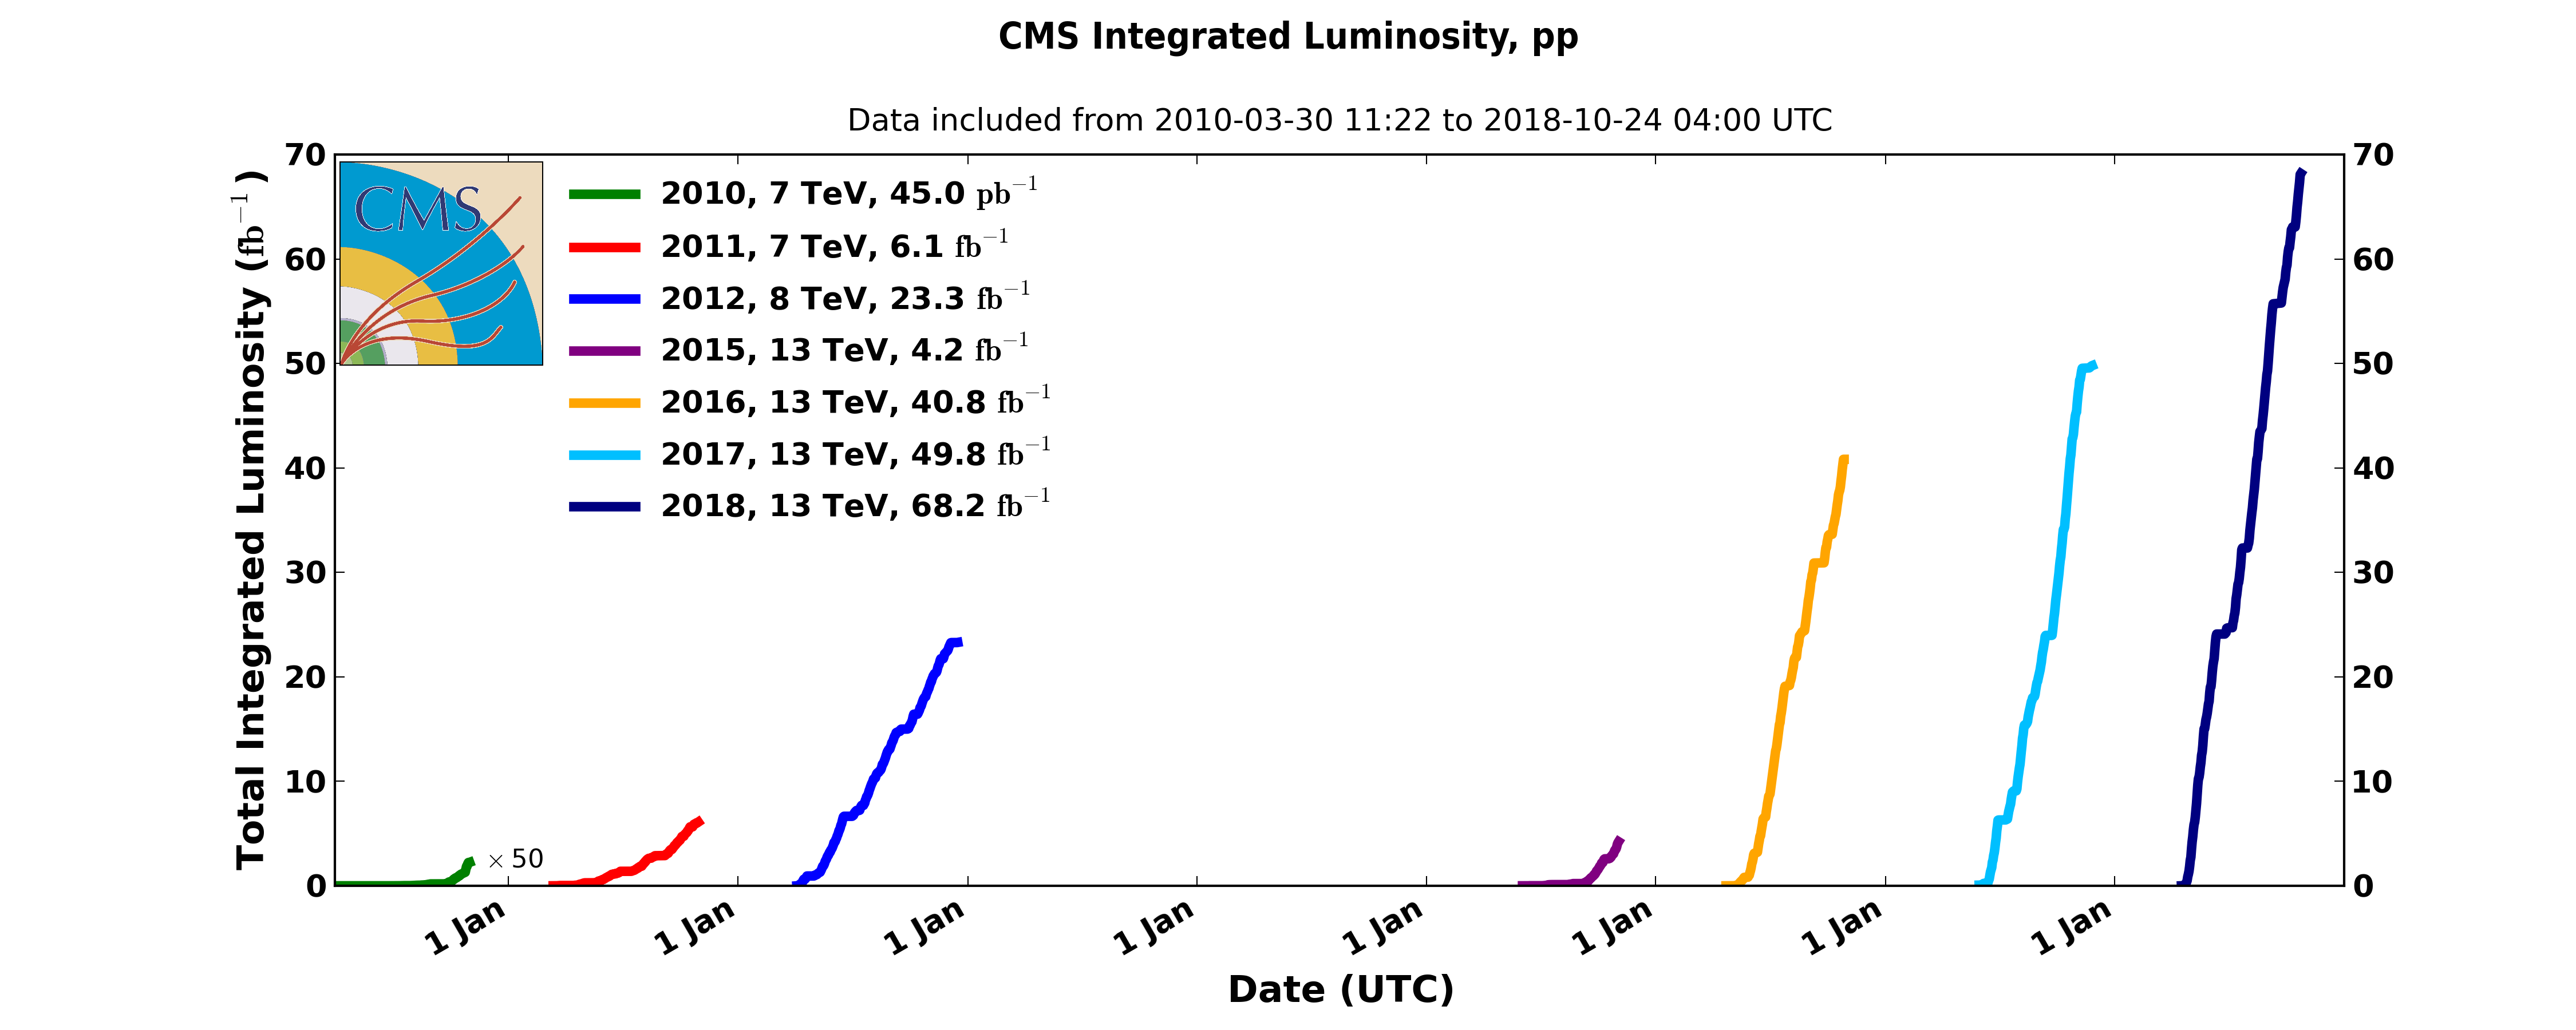
\includegraphics[scale= 0.4]{../Cap2/int_lumi_cumulative_pp_1}
\caption{Run-I ans Run-II integrated luminosity.}
\label{int_lumi_cumulative_pp_1}
\end{figure}
In 2017 and 2018 operations continued and the total integrated luminosity for Run-II is now around $\sim$150 fb$^{-1}$. 
In October 2018 the protons collisions have been stopped, Fig.~\ref{beam}, and all operation (ions collisions after the proton stop) will  halt in 2019 for a second long shutdown of $\sim$2.5 year (LS2) for the machine and experiments upgrade. The Run-III will start in 2021 with an energy of 14 TeV.
After that,  as shown in Fig.~\ref{lhcplan}, the third long shutdown (LS3) starting in 2024, will see a
substantial upgrade of the LHC and of both Atlas and CMS experiments.
The high-luminosity LHC (HL-LHC) starting in $\sim$2026
will represent an unprecedented way to study very rare phenomena at the LHC. The
machine is expected to deliver, during a decade of operations, an integrated luminosity
of $\sim$3000~fb$^{-1}$.
\begin{figure}
\centering
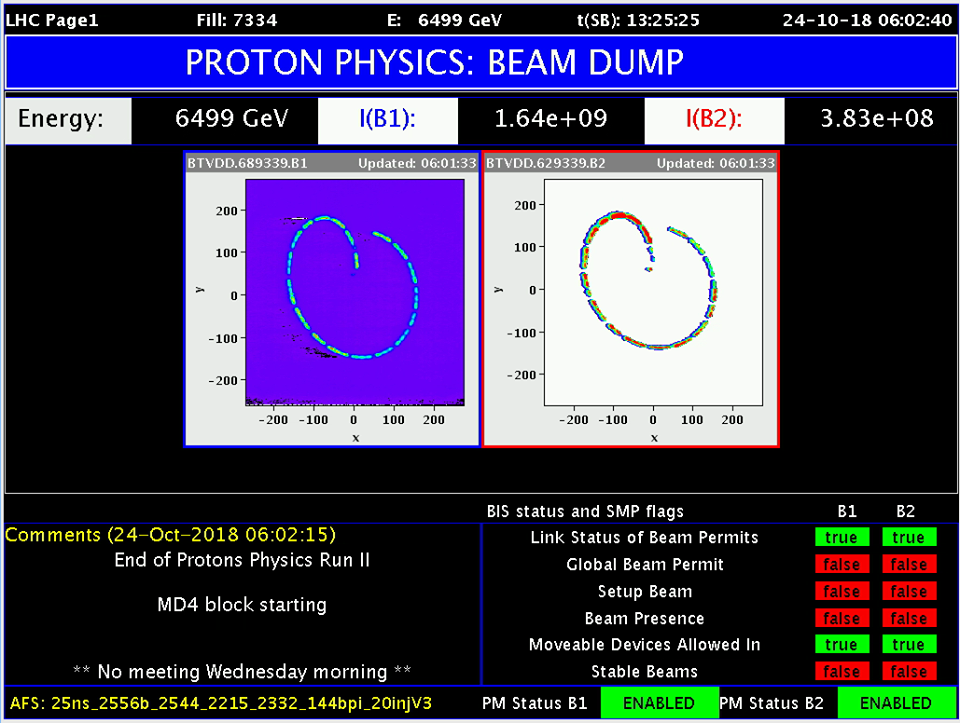
\includegraphics[scale= 0.2]{../Cap2/beam}
\caption{Last proton-proton beam dump at the end of Run-II.}
\label{beam}
\end{figure}
\begin{figure}
\centering
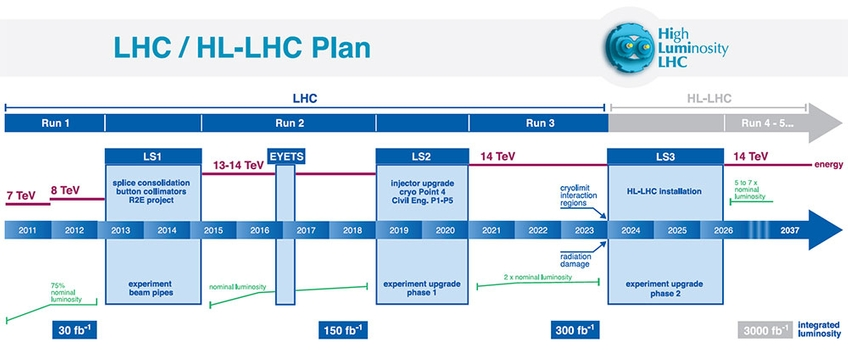
\includegraphics[scale= 0.5]{../Cap2/lhcplan}
\caption{Schedule of LHC and HL-LHC operations.}
\label{lhcplan}
\end{figure}





